\chapter{Balanced Search Tree}
\section{2-3 Search Tree}
\subsection{Insertion}
Insertion into a 3-node at bottom:
\begin{enumerate}
\item Add new key to the 3-node to create a temporary 4-node.
\item Move middle key of the 4-node into the parent (including root's parent).
\item Split the modified 4-node.
\item Repeat recursively up the trees as necessary.
\end{enumerate}
\begin{figure}[hbtp]
\centering
\subfloat{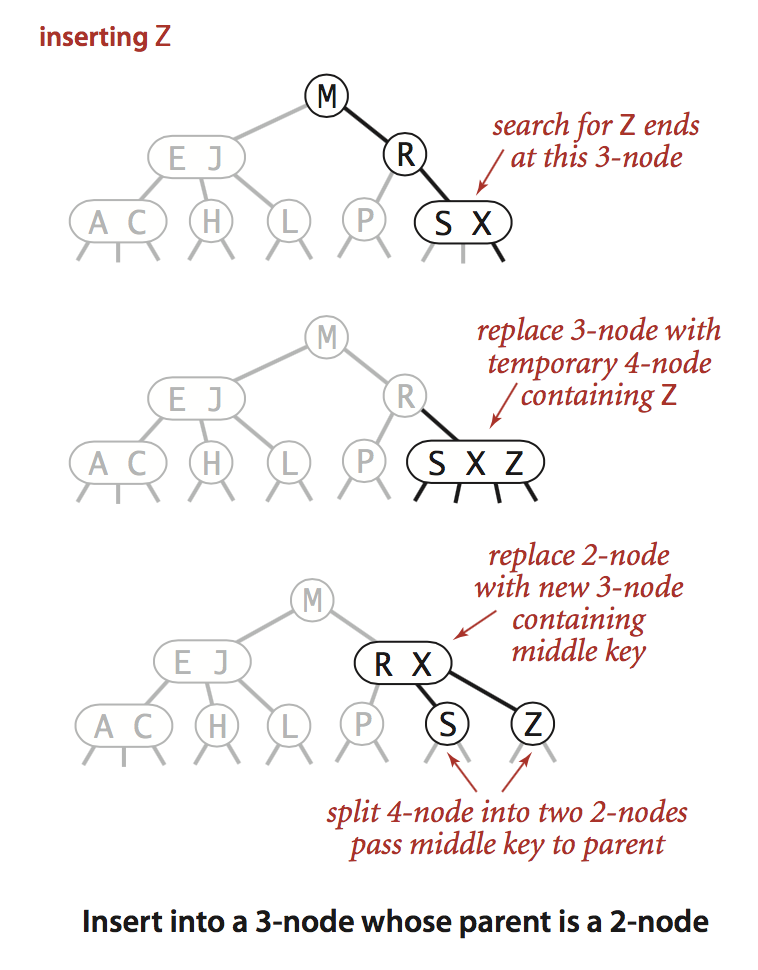
\includegraphics[scale=1.]{23insert1}}
\caption{Insertion 1}
\label{fig:LABEL}
\end{figure}

\begin{figure}[hbtp]
\centering
\subfloat{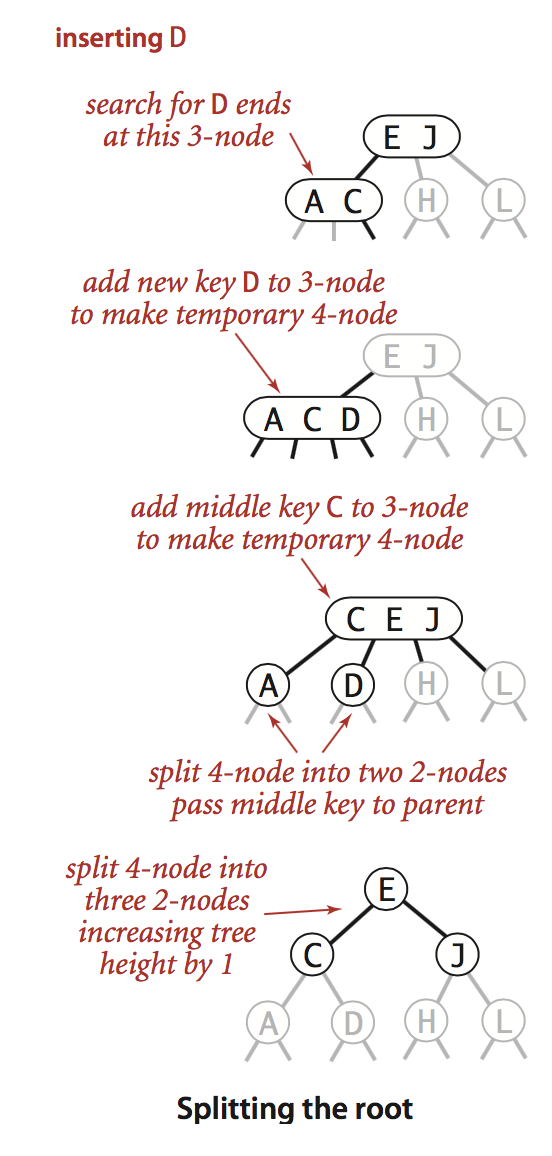
\includegraphics[scale=1.]{23insert2}}
\caption{insert 2}
\label{fig:LABEL}
\end{figure}

\subsection{Splitting}
Summary of splitting the tree. 
\begin{figure}[hbtp]
\centering
\subfloat{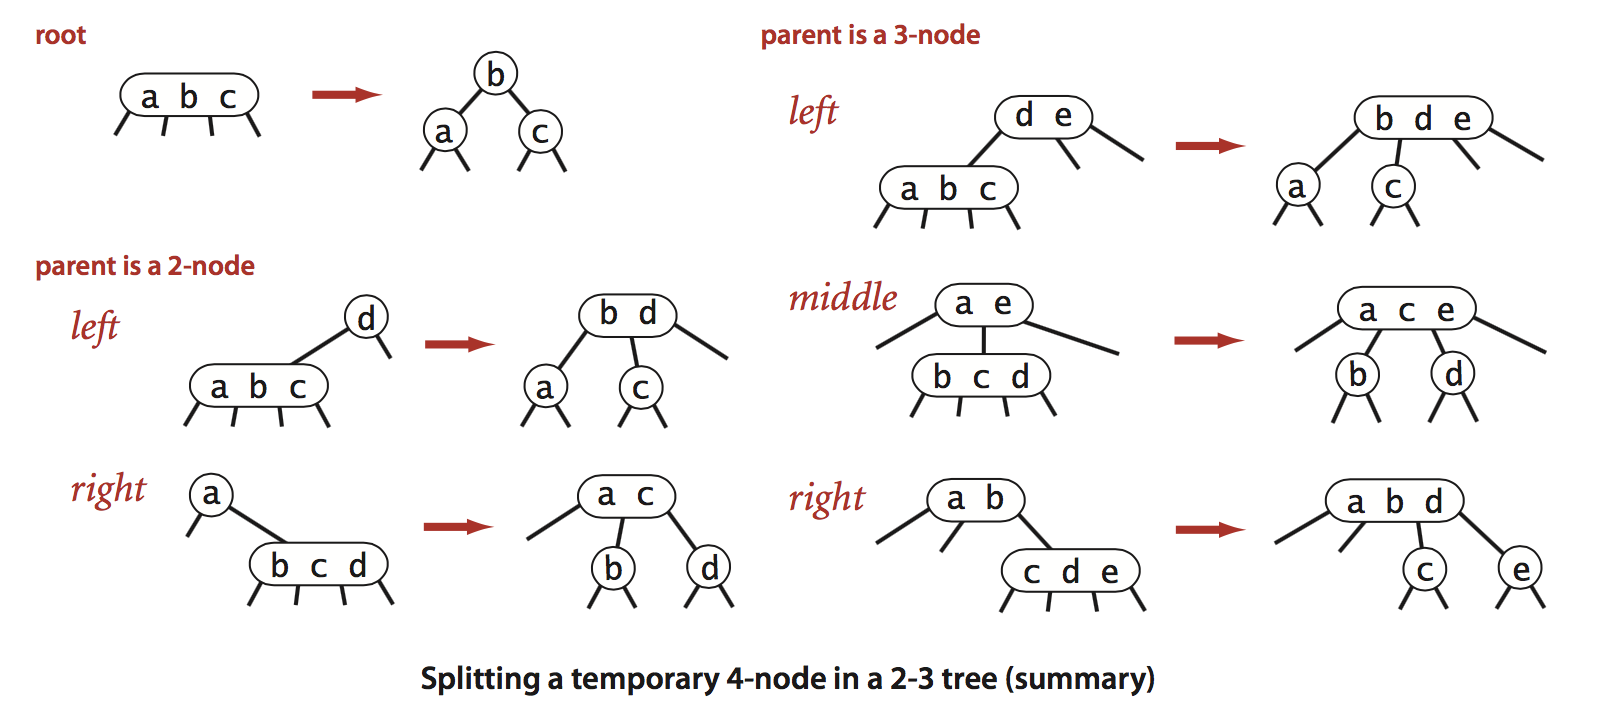
\includegraphics[scale=.60]{23splitting}}
\caption{Splitting temporary 4-ndoe summary}
\label{fig:splitting}
\end{figure}

\subsection{Properties}
When inserting a new key into a 2-3 tree, under which one of the following scenarios must the height of the 2-3 tree increase by one? When every node on the search path from the root is a 3-node

\section{Red-Black Tree}
\subsection{Properties}
Red-black tree is an implementation of 2-3 tree using \textbf{leaning-left red link}. \begin{figure}[hbtp]
\centering
\subfloat{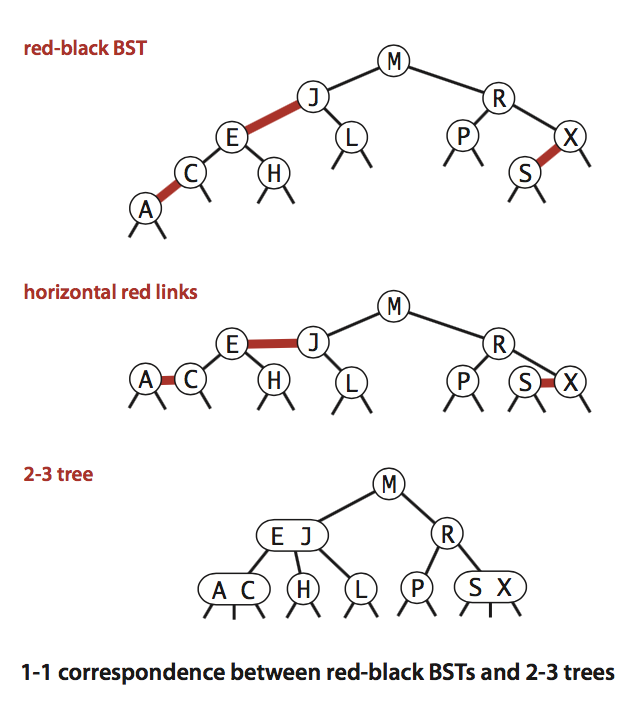
\includegraphics[scale=1.1]{rbtree11}}
\caption{RB-tree and 2-3 tree}
\label{fig:LABEL}
\end{figure}
The hight of the RB-tree is at most $2\lg N$ where alternating red and black links.

\runinhead{Perfect black balance.}Every path from root to null link has the same number of black links.
\subsection{Operations}
\runinhead{Elementary operations:}
\begin{enumerate}
\item Left rotation: orient a (temporarily) right-leaning red link to lean left.
\item Right rotation: orient a (temporarily) left-leaning red link to lean right. 
\item Color flip: Recolor to split a (temporary) 4-node. 
\end{enumerate}
\begin{figure}[hbtp]
\centering
\subfloat{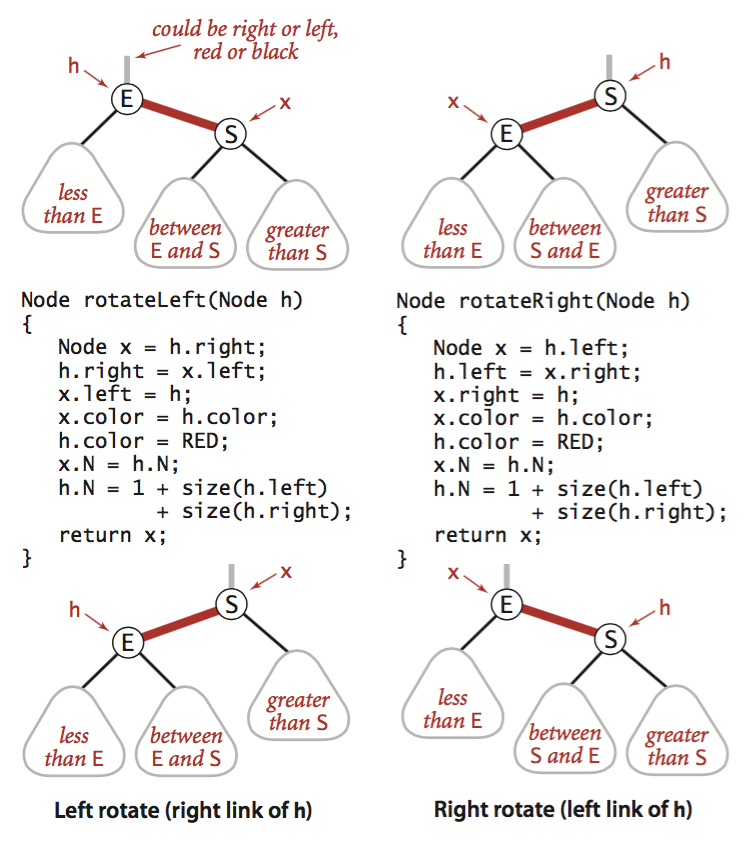
\includegraphics[scale=1.20]{rbrotate}}
\caption{Rotate left/right}
\label{fig:LABEL}
\end{figure}

\begin{figure}[hbtp]
\centering
\subfloat{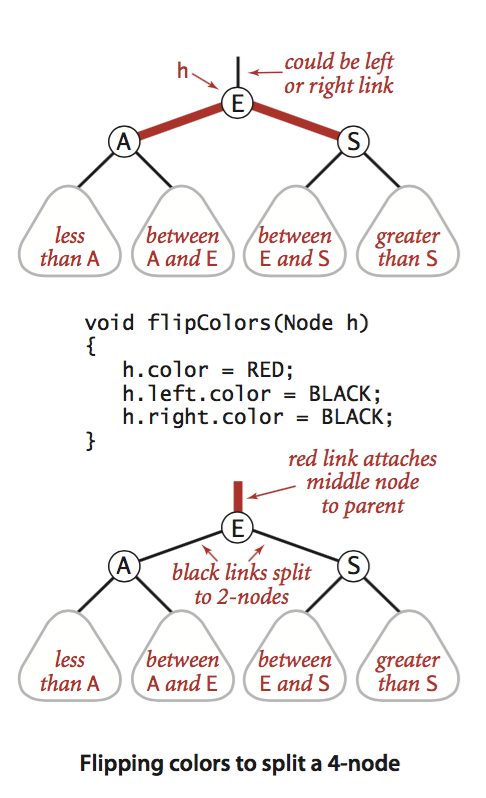
\includegraphics[scale=1.20]{rbflip}}
\caption{Flip colors}
\label{fig:LABEL}
\end{figure}

\runinhead{Insertion.} When doing insertion, from the child's perspective, need to have the information of current leaning direction and parent's color. Or from the parent's perspective - need to have the information of children's and grandchildren's color and directions.

For every new insertion, the node is always attached with red links. 
\begin{java}
Node put(Node h, Key key, Value val) {
    if (h == null)  // Do standard insert, with red link to parent.
       return new Node(key, val, 1, RED);
    int cmp = key.compareTo(h.key);
    if      (cmp < 0) h.left  = put(h.left,  key, val);
    else if (cmp > 0) h.right = put(h.right, key, val);
    else h.val = val;
    if (isRed(h.right) && !isRed(h.left))    h = rotateLeft(h);
    if (isRed(h.left) && isRed(h.left.left)) h = rotateRight(h);
    if (isRed(h.left) && isRed(h.right))     flipColors(h);
    h.N = 1+size(h.left)+size(h.right);
    return h; 
}
\end{java}

\runinhead{Deletion.} Deletion is more complicated. 

\section{B-Tree}


\section{AVL Tree}
